This chapter aims to describe fundamental relationships between combinatorial optimization problems 
and linear programming. More specifically, we will define a new problem -- the vertex cover problem -- 
and show how this problem is intimately related to the matching problem. The way we show this 
relationship is through duality theory. We also use this to shed light on the max-flow/min-cut 
theorem.

\begin{section}{The vertex cover problem}
	We begin this section by defininig a new problem. Again, this is a problem on graphs in 
	general, but we will be restricting our attention to bipartite graphs. This is a good idea 
	for many reasons, but the most pertinent reason is that this problem is NP-complete in the 
	general case.

	\begin{definition}
		Let $G = (U,V,E)$ be a bipartite graph. A subset $C\subset U\cup V$ is said to be a 
		\emph{vertex cover} if for each $(u,v)\in E$ we have that at least one of $u,v \in C$.
		$C$ is a \emph{minimum} vertex cover if for any other cover $C\'$, $|C|\leq |C\'|$.
	\end{definition}
	Using what we've already learned, we can specify at least one relation between matchings and 
	vertex covers: namely, the set of all vertices of all edges in any maximal matching on a graph 
	forms a vertex cover. Figure 1 shows some examples of vertex covers on the graph we looked at 
	in the previous chapter.

	\begin{figure}[h]
		\centering
		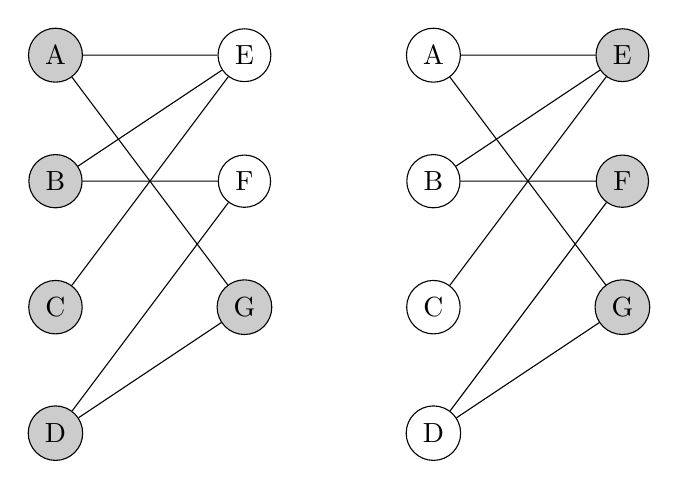
\begin{tikzpicture}[scale=.8,auto=left,every node/.style={circle,draw=black}]
		
		%left nodes
		\node[fill=black!20] (n1) at (1,10) {A};
		\node[fill=black!20] (n2) at (1,8) {B};
		\node[fill=black!20] (n3) at (1,6) {C};
		\node[fill=black!20] (n4) at (1,4) {D};

		%right nodes
		\node (n5) at (4,10) {E};
		\node (n6) at (4, 8) {F};
		\node[fill=black!20] (n7) at (4, 6) {G};
		
		%edges
		\draw (n1) -- (n5);
		\draw (n1) -- (n7);
		\draw (n2) -- (n5);
		\draw (n2) -- (n6);
		\draw (n3) -- (n5);
		\draw (n4) -- (n6);
		\draw (n4) -- (n7);

		%left nodes
		\node (m1) at (7,10) {A};
		\node (m2) at (7,8) {B};
		\node (m3) at (7,6) {C};
		\node (m4) at (7,4) {D};

		%right nodes
		\node[fill=black!20] (m5) at (10,10) {E};
		\node[fill=black!20] (m6) at (10, 8) {F};
		\node[fill=black!20] (m7) at (10, 6) {G};
		
		%edges
		\draw (m1) -- (m5);
		\draw (m1) -- (m7);
		\draw (m2) -- (m5);
		\draw (m2) -- (m6);
		\draw (m3) -- (m5);
		\draw (m4) -- (m6);
		\draw (m4) -- (m7);

		\end{tikzpicture}
		\caption{Examples of vertex covers}
	\end{figure}
	You can convince yourself that the cover on the right is a minimum cover. This brings us 
	to an important theorem. We first prove a lemma.

	\begin{lemma}
		Let $G=(U,V,E)$ be a bipartite graph. Let $M$ be a matching on $G$ and $C$ a cover on 
		$G$ such that $|M| = |C|$. Then $M$ is a maximum matching and $C$ is a minimum 
		covering.
	\end{lemma}

	\begin{proof}
		Let $M\'$ be a maximum matching on $G$ and $C\'$ a minimum covering on $G$. For each 
		$(u,v)\in M\'$, $C\'$ must include either $u$ or $v$, which tells us that 
		$|M\'| \leq |C\'|$. Then we have 
		\[
			|M|\leq |M\'| \leq |C\'| \leq |C|.
		\]
		Thus, if $|M| = |C|$ we have equalities above, which means that the size of a maximum 
		matching is equal to the size of a minimum covering.
	\end{proof}

	\begin{theorem}{(K\H{o}nig-Egervary)}
		For any bipartite graph $G$, if $M$ is a maximum matching on $G$ and $C$ is a minimum 
		vertex cover  on $G$, then $|M| = |C|$.
	\end{theorem}
	Before we prove this, we define a simple term: an $M$-alternating path is an alternating path 
	with respect to a matching $M$.
	\begin{proof}
		Let $G=(U,V,E)$ be a bipartite graph, and let $M$ be a maximum matching on $G$. 
		Furthermore, define
		\begin{align}
			A &:= \{s\in S\; |\; s \text{ unmatched}\}\\
			B &:= \{\text{all vertices connected to nodes in $A$ by $M$-alternating paths}\}.
		\end{align}
		Let $L = B\cap U$ and $R = B\cap V$. Then we have the following:
		\begin{enumerate}
			\item Every node in $R$ is saturated.
			\item $N(L) = R$,
		\end{enumerate}
		where $N(L)$ denotes the set of all vertices connected to elements of $L$ (the 
		``neighbors'' of $L$). The first claim comes from the fact that, if $M$ is a 
		maximum matching, then our alternating paths starting at nodes in $A$ must have 
		length $\geq 2$, and must have even length (otherwise we would have an augmenting path, 
		which contradicts our assumption that $M$ is a maximum matching).
		The second comes from that fact that every node in $N(L)$ is connected to vertices in 
		$A$ by an alternating path. \\
		Now, define $K := (U\setminus L)\cup R$. Every edge 
		in $G$ must have one of its endpoints in $K$. If not, there there would be an 
		edge with one end in $L$ and one end in $V\setminus R$, which contradicts 
		$N(L) = R$. So $K$ is a covering of $G$. Moreover, $|K| = |M|$, since for each 
		edge in $M$ we've included one of its endpoints in $K$ (the vertices we've chosen are 
		those in $N(L)$ and those in $U\setminus L$). Thus, by the previous lemma, $K$ is 
		a minimum covering.
	\end{proof}
	All of this tells us that there is a deep relationship between maximum matchings and 
	minimum vertex covers on bipartite graphs. Given a solution to one, we can turn it into a 
	solution to the other. This is what we seek to accomplish next. 
\end{section}

\begin{section}{Duality theory}
	\begin{definition}
		Let 
		\begin{alignat*}{2}
			& \text{maximize } & \mathbf{c}^{T}\mathbf{x} \\
			& \text{subject to } & A\mathbf{x} & \leq \mathbf{b} \\
			&& \mathbf{x} &\geq 0
		\end{alignat*}
		be our linear program, which we will call the \emph{primal} linear program. Then we 
		define the \emph{dual} of this linear program to be the linear program
		\begin{alignat*}{2}
			& \text{minimize } & \mathbf{b}^{T}\mathbf{y} \\
			& \text{subject to } & A^{T}\mathbf{y} & \leq \mathbf{c} \\
			&& \mathbf{y} &\geq 0
		\end{alignat*}
	\end{definition}
	The first thing to note is that the dual of the dual is the primal. Let us introduce some 
	notation. First, let us denote the primal maximization problem by the letter $\Gamma$, and 
	the dual minimization problem by the letter $\Omega$. For a given linear program, we denote 
	an optimal solution by $\mathbf{OPT}$. 

	\begin{theorem}{(Weak duality)}
		If the primal linear program (in maximization form) and the dual (in minimization 
		form) are both feasible, then 
		\[
			\mathbf{OPT}(\Gamma) \leq \mathbf{OPT}(\Omega).
		\]
	\end{theorem}
	What's surprising is the following theorem.

	\begin{theorem}{(Strong duality)}
		Given two linear programs $\Gamma$ and $\Omega$ that are duals of each other, if one is 
		feasible and bounded, then so is the other. Additionally, 
		\[
			\mathbf{OPT}(\Gamma) = \mathbf{OPT}(\Omega).
		\]
	\end{theorem}
	Our goal now is to use this duality theory to better understand the relationships between 
	our combinatorial optimization problems.

\begin{subsection}{Maximum-matching duality}
	Let's first turn maximum matching into a linear program. Our goal is to maximize the number 
	of edges in our matching. Our constraint is that no edge is incident to more than one edge 
	in the matching. So for each edge $(u,v)$, we will need a corresponding $x_{uv}$. Our objective 
	function is then pretty simple: maximize the number of $x_{uv}$. Now we need to figure out 
	our constraint equations. For a fixed node $u\in U$, the number of edges in the matching 
	incident 
	to $u$ is given by $\sum_{v\in V} x_{uv}$. So we want that this is $\leq 1$. Similarly, for any 
	node $v$, we want $\sum_{u\in U} x_{uv} \leq 1$. This gives us the following linear program.
	\begin{alignat}{3}
		& \text{maximize } & \sum_{u,v} x_{uv}& \\
		& \text{subject to } \quad & \sum_{v} x_{uv} & \leq 1, & \quad \forall u\in U&, \\
				     &\quad & \sum_{u} x_{uv} & \leq 1, & \quad \forall v\in V &, \\
				&& x_{uv} & \in \{0,1\}.
	\end{alignat}
	What we've given here is an $\emph{integer}$ linear program, since we've restricted our 
	$x$ variables to be integers. In general, solving integer linear programs is NP-hard. However, 
	in this case it is well know that this linear program attains integer solution at extreme 
	of the polyhedron solution space, so we can drop the integrality requirements and just say 
	$x_{uv} \geq 0$.\\
	Now let's try and construct the dual of this linear program. We will need a variable 
	$y_u$ for each vertex $u$. Similarly, we need a variable $y_v$ for each vertex $v$. Our 
	objective will be to minimize over the sum of these $y_u,y_v$. Since our constraint 
	in the primal is the constant vector 1, our only constraint will be that $y_u + y_v \geq 1$. 
	This gives us the dual linear program
	\begin{alignat}{3}
		& \text{minimize } & \sum_{u,v} (y_u + y_v)& \\
		& \text{subject to } \quad & y_u + y_v & \geq 1 & \quad \forall u,v &, \\
				    && y_u,y_v & \geq 0.
	\end{alignat}
	This dual problem tells us that each edge must be ``covered'' by at least one of its incident 
	vertices. This is exactly the vertex cover problem! So for unweighted bipartite graphs, the 
	linear programs for maximum matchings and minimum vertex covers are duals of each other. 
	We will use this insight to construct our algorithms for solving the maximum matching problem. 
	\\
	There is another version of this problem, called the \emph{maximum weight matching}. In this 
	version, we are given a bipartite graph with non-negative edge weights $w_{uv}$ for all 
	edges $(u,v)$. Instead of trying to maximize the number of edges in the matching, the goal 
	is to find a matching $M$ such that $\sum_{(u,v) \in M} w_{uv}$, or the weight of the matching, 
	is greater than the weight of any other matching. We can easily encode this problem by making 
	a slight modification to our linear program from before. The primal is given by
	\begin{alignat}{3}
		& \text{maximize } & \sum_{u,v} w_{uv}x_{uv}& \\
		& \text{subject to } \quad & \sum_{v} x_{uv} & \leq 1, & \quad \forall u\in U&, \\
				     &\quad & \sum_{u} x_{uv} & \leq 1, & \quad \forall v\in V &, \\
				&& x_{uv} & \geq 0.
	\end{alignat}
	Then the dual is
	\begin{alignat}{3}
		& \text{minimize } & \sum_{u} y_u + \sum_v y_v& \\
		& \text{subject to } \quad & y_u + y_v & \geq w_{uv} & \quad \forall u,v &, \\
				    && y_u,y_v & \geq 0.
	\end{alignat}
	The dual is a sort of weighted vertex cover. One way to think about it is that each edge 
	has a ``cost'' given by $w_{uv}$, and each of its endpoints has to pool ``money'' in order 
	to pay at least that cost. So instead of edges being covered or not covered, there's a certain 
	``amount'' that they have to be covered.
\end{subsection}

\begin{subsection}{Revisiting a familiar problem - max-flow/min-cut}
	Here we demonstrate that a common problem discussed in algorithms courses, and a quite 
	amazing theorem, is really a special case of what we've been discussing. Recall that a 
	flow network is defined as follows.
	\begin{definition}
		A \emph{flow network} $G = (V,E)$ is a directed graph in which each edge $(u,v)\in E$ 
		has nonnegative \emph{capacity} $c_{uv} \geq 0$. Furthermore, there are two 
		vertices, a source $s$ and a sink $t$. We assume that every $v\in V$ lies in 
		some path $s\to \cdots \to v\to \cdots \to t$.
	\end{definition}
	\begin{definition}
		Let $G = (V,E)$ be a flow network. A \emph{flow} in $G$ is a function $f: V\times V \to 
		\R$ that satisfies the following:
		\begin{itemize}
			\item Capacity constraint: For all $u,v\in V$, $0\leq f(u,v) \leq 
				c_{uv}$.
			\item Conservation: For all $u\in V\setminus \{s,t\}$, we have 
				\[
					\sum _{v\in V} f(v,u) = \sum_{v\in V} f(u,v).
				\]
				This says that for all vertices $v$ except our source and sink, the 
				flow out of $v$ is equal to the flow into $v$. 
		\end{itemize}
		We define the value of the flow $val(f) = \sum_{v\in V} f(s,v) - \sum_{v\in V} f(v,s)$, 
		which is just the flow out of our source minus the flow into our source.
	\end{definition}
	The problem as demonstrated in a typical algorithms course is to find a maximum flow from $s$ 
	to $t$. This is done using a method developed by Ford and Fulkerson which does what $ALG 1$ 
	does, but in a residual graph (essentially the subgraph where the flows $f(u,v) < c_{uv}$, we 
	refer the reader to [CITE CLRS] for more detail). \\
	Now, we recal the definition of a cut in a flow network.
	\begin{definition}
		A \emph{cut} $(S,T)$ of a flow network $G=(V,E)$ is a partition of $V$ into sets $S$ 
		and $T = V\setminus S$ such that $s\in S$ and $t\in T$. Given a flow $f$, the 
		\emph{net flow} $f(S,T)$ across the cut $(S,T)$ is defined as 
		\[
			f(S,T) = \sum_{u\in S} \sum_{v\in T} f(u,v) - \sum_{u\in S} \sum_{v\in T} 
			f(v,u).
		\]
		Finally, the \emph{capacity} of the cut is $c(S,T) = 
		\sum_{u\in S} \sum_{v\in T} c(u,v)$. A minimum cut has capacity less than or equal to 
		all other cuts in the network/
	\end{definition}
	One of the coolest and most surpising theorems in an algorithms corse is that, given a flow 
	network $G$, the value of the maximum flow ($val(f)$) is equal to the capacity of the minimum 
	$s-t$ cut of $G$.

	Our goal now is to build up to this same theorem using the tools developed in this chapter. 
	What follows is due to [CITE VAZIRANI]. We will first give a linear program for the 
	maximum flow problem. To make things simpler, let's introduce an arc of infinite capacity 
	from the sink $t$ to the source $s$; this converts this to a circulation, with the objective to 
	maximize the flow $f(t,s)$. This allows us to enforce flow conservation at $s$ and $t$ as well, 
	which makes the corresponding linear program simpler. The linear program is as follows.
	\begin{alignat*}{3}
		& \text{maximize } & f(t,s)\\
		& \text{subject to } & f(u,v) &\leq c_{uv}, &\quad (u,v)\in E\\ 
				     && \sum_{v:(v,u)\in E} f(v,u) & \leq \sum_{v:(u,v)\in E} f(u,v), &
				     	\quad u\in V &\\
				     && f(u,v) &\geq 0 &\quad (u,v)\in E &.
	\end{alignat*}
	It is not immediately obvious why the second set of inequalities implies flow conservation; all 
	it seems to say is that for each $u$, the total flow into $u$ is at most the total flow out 
	of $u$. However, note that if this holds for all $u$, we in fact have equality of incoming and 
	outgoing flow, since a deficit of flow at some $u$ implies a flow surplus at some $v$. So 
	this does in fact give us conservation of flow. Now we want to find the dual of this program. 
	Our sense (hopefully) is that the dual will somehow relate to minimum cuts, given the 
	foreshadowing of the previous section. Let's see! We introduce variables $d_{uv}$ and $p_u$ for 
	each type of inequality in the primal.
	\begin{alignat*}{3}
		& \text{minimize } & \sum_{(u,v)\in E} c_{uv} d_{uv}& \\
		& \text{subject to } \quad & d_{uv} - p_u + p_v & \geq 0, & \quad (u,v)\in E &, \\
				    && p_s - p_t & \geq 1, & \\
				    && d_{uv} & \geq 0, & \quad (u,v) \in E &.
	\end{alignat*}
	It is known that extreme point solutions to these linear programs takes on values 0 or 1 at 
	each coordinate. Let consider an optimal dual solution $(\mathbf{d}^{*},\mathbf{p}^{*})$. 
	First, in order to satisfy $p_s^{*} - p_{t}^{*} \geq 1$ with 0,1 values, it must be the case 
	that $p_s^{*} = 1$ and $p_t^{*} = 0$. This motivates an $s-t$ cut $(S,T)$ with $S$ consisting 
	of nodes with value 1, and $T$ the nodes with value zero. For an edge $(u,v)$ such that 
	$u\in S$ and $v\in T$, we have that $p_u^{*} = 1$ and $p_v^{*} = 0$, so by the first constraint 
	$d_{uv}^{*} = 1$. This means that for any edge $(u,v)$ in the cut, the corresponding 
	$d_{uv}^{*} = 1$. Note that any other $d_{uv}^{*}$ where $(u,v)$ is not in the cut, it's value 
	can be 0 without violating the constraints (we want them to be 0 since we are minimizing our 
	objective function). Thus the objective function's value is equal to the capacity of this 
	$(S,T)$ cut, which must be a minimum cut. Strong duality tells us that this corresponds to the 
	value of $f(t,s)$ in the primal linear program. To make this clear, we give an example of a 
	flow network.\\
	\begin{figure}[H]
		\centering
		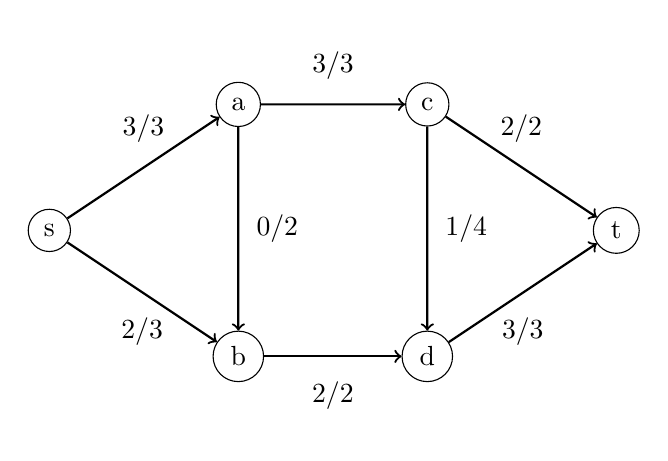
\begin{tikzpicture}[scale=.8,auto=left,every node/.style={circle,draw=black}]
			\node (n1) at (3,3) {s};
			\node (n2) at (6,5) {a};
			\node (n3) at (6,1) {b};
			\node (n4) at (9,5) {c};
			\node (n5) at (9,1) {d};
			\node (n6) at (12,3) {t};

			\draw[->,thick] (n1) -- node[draw=none, above] {3/3} ++ (n2);
			\draw[->,thick] (n1) -- node[draw=none, below] {2/3} ++ (n3);
			\draw[->,thick] (n2) -- node[draw=none, right] {0/2} ++ (n3);
			\draw[->,thick] (n2) -- node[draw=none, above] {3/3} ++ (n4);
			\draw[->,thick] (n3) -- node[draw=none, below] {2/2} ++ (n5);
			\draw[->,thick] (n4) -- node[draw=none, right] {1/4} ++ (n5);
			\draw[->,thick] (n4) -- node[draw=none, above] {2/2} ++ (n6);
			\draw[->,thick] (n5) -- node[draw=none, below] {3/3} ++ (n6);
		\end{tikzpicture}
		\caption{Flow network with maximum flow of 5}
	\end{figure}
	In Figure 2.2 we have a flow network that has a maximum flow from $s$ to $t$ of 5. We should 
	expect that, given our discussion of the dual, we shoul be able to find a cut $(S,T)$ of value 5 
	such that $S$ consists of nodes with value 1, and $T$ consists of nodes with value 0. We know 
	that we must set $p_s = 1$ and $p_t = 0$. This gives us the following dual solution, where grey 
	nodes are in $S$ and white nodes are in $T$.\\
	\begin{figure}[H]
		\centering
		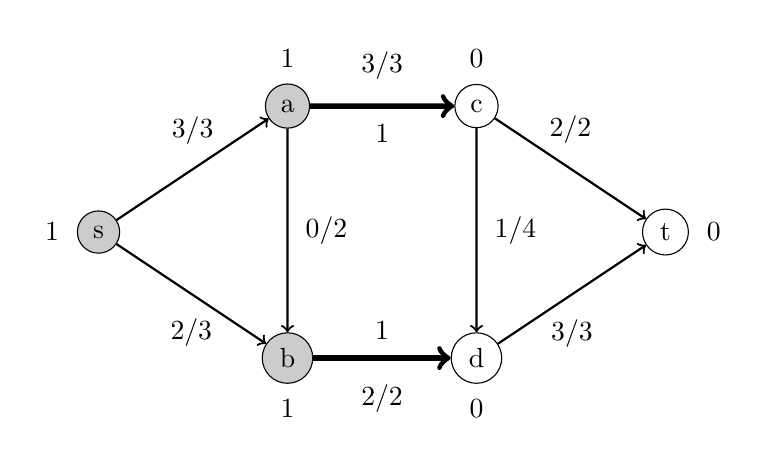
\begin{tikzpicture}[scale=.8,auto=left,every node/.style={circle,draw=black}]
			\node [fill=black!20, label=left:{1}] (n1) at (3,3) {s};
			\node [fill=black!20, label=above:{1}] (n2) at (6,5) {a};
			\node [fill=black!20, label=below:{1}] (n3) at (6,1) {b};
			\node [label=above:{0}] (n4) at (9,5) {c};
			\node [label=below:{0}] (n5) at (9,1) {d};
			\node [label=right:{0}] (n6) at (12,3) {t};

			\draw[->,thick] (n1) -- node[draw=none, above] {3/3} ++ (n2);
			\draw[->,thick] (n1) -- node[draw=none, below] {2/3} ++ (n3);
			\draw[->,thick] (n2) -- node[draw=none, right] {0/2} ++ (n3);
			\draw[->,line width=0.7mm] (n2) -- node[draw=none, above] {3/3} 
			node[draw=none, below] {1} ++ (n4);
			\draw[->,line width=0.7mm] (n3) -- node[draw=none, below] {2/2} 
			node[draw=none, above] {1} ++ (n5);
			\draw[->,thick] (n4) -- node[draw=none, right] {1/4} ++ (n5);
			\draw[->,thick] (n4) -- node[draw=none, above] {2/2} ++ (n6);
			\draw[->,thick] (n5) -- node[draw=none, below] {3/3} ++ (n6);
		\end{tikzpicture}
		\caption{Flow network with corresponding dual solution}
	\end{figure}
	In Figure 2.3, the $(S,T)$ cut corresponds to the sets $S= \{s,a,b\}$ and $T = \{c,d,t\}$; the 
	edges in the cut are the bold edges $a\to c$ and $b\to d$. So the capacity of the cut is 5, 
	which is what we'd expect. In order to make the figure readable, we leave out our dual labeling 
	on edges that are not in the cut (their label is 0 anyways). The label on edges in the cut is 
	1, which we leave in. Note that our dual labeling of edges and vertices in this flow network 
	satisfies our dual constraints.\\
	Thus, we have given an alternative formulation of the max-flow/min-cut relationship using 
	linear programs. In this next chapter we present the main algorithm of this thesis, the 
	Hungarian algorithm, which is interesting in itself, and also as a tool to motivate general 
	primal-dual algorithms.
\end{subsection}
\end{section}
